\documentclass[../thesis/thesis.tex]{subfiles}
\begin{document}
\chapter{Literature Review}
\label{chap:litreview}

% TODO: Actually talk about how well existing solutions fit
Within this chapter we consider the broad variety of sensing systems available, and how well different types of sensors meet our sensing criteria. It can be difficult to approach the board variety of sensor types in the field, so a structure must be developed through which to evaluate them. Teixeira, Dublon and Savvides \cite{teixeira2010survey} propose a 5-element human-sensing criteria which provides a structure through which we may define the broad quantitative requirements of different sensors.

These quantitative requirements can be used to exclude sensing options that clearly cannot meet the requirements before the more specific qualitative accessibility criteria will be considered for those remaining sensors. 

The quantitative criteria elements are;
\begin{enumerate}
 \item \emph{Presence}: Is there any occupant present in the sensed area?
 \item \emph{Count}: How many occupants are there in the sensed area?
 \item \emph{Location}: Where are the occupants in the sensed area?
 \item \emph{Track}: Where do the occupants move in the sensed area? (local identification)
 \item \emph{Identity}: Who are the occupants in the sensed area? (global identification)
\end{enumerate}

At a fundamental level, this research project requires a sensor system that provides both Presence and Count information. To assist with the reduction of privacy concerns, excluding systems that permit Identity information will generally result in a less invasive system also. The presence of Location or Track information are irrelevant to our project's goals, but overall, minimizing these elements should in most cases help to maximize the energy efficiency of the system also.

Teixeira, Dublon and Savvides \cite{teixeira2010survey} also propose an occupancy sensor taxonomy (see \Fref{fig:litreview:taxonomy}), which categorizes different sensing systems in terms of what information they use as a proxy for human-sensing. We use this taxonomy here as a structure through which we group and discuss different sensor types.

\begin{figure}
\centering
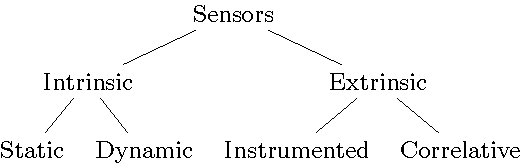
\includegraphics{../diagrams/category-tree.pdf}
\caption{Taxonomy of occupancy sensors}
\label{fig:litreview:taxonomy}
\end{figure}

\section{Intrinsic traits}
\label{subsec:litreview:sensors:intrinsic}

Intrinsic traits are those which can be sensed that are a direct property of being a human occupant. Intrinsic traits are particularly useful, as in many instances they are guaranteed to be present if an occupant is present. However, they do have varying degrees of detectability and differentiation between occupants. Two main subcategories of these sensor types are static and dynamic traits.

\subsection{Static traits}
\label{subsubsec:litreview:sensors:intrinsic:static}
Static traits are physiologically derived, and are present with most (living) occupants. One key static trait that can be used for occupant sensing is that of thermal emissions. All human occupants emit distinctive thermal radiation in both resting and active states. The heat signatures of these emissions could potentially be measured with some apparatus, counted, and used to provide Presence and Count information to a sensor system, without providing Identity information.

Beltran, Erickson and Cerpa \cite{beltran2013thermosense} propose Thermosense, a system that uses a type of thermal sensor known as a \iar. This sensor is much like a camera, in that it has a field of view which is divided into ``pixels''; in this case an $8\times8$ grid of detected temperatures. This sensor is mounted on an embedded device on the ceiling, along with a \pir for basic motion detection, and uses machine learning algorithms to detect human heat signatures within the raw thermal and motion data it collects. Thermosense measures accuracy with Root Mean Squared Error (RMSE), an average of the absolute value that their prediction deviated from the true result.

Another static trait is that of \cdi emissions, which, like thermal emissions, are emitted by human occupants in both resting and active states. By measuring the buildup of \cdi within a given area, one can use a variety of mathematical models of human \cdi production to determine the likely number of occupants present. Hailemariam \etal \cite{hailemariam2011real} trialled this as part of a sensor fusion within the context of an office environment, achieving a $\approx94\%$ accuracy. Such a sensing system could provide both the Presence and Count information, and exclude the Identity information as required. However, \cdi based detection methods have serious drawbacks, discussed by Fisk, Faulkner and Sullivan \cite{fisk2006accuracy}: The \cdi feedback mechanism is very slow, taking hours of continuous occupancy to correctly identify the presence of people. In a residential environment, occupants are more likely to be moving between rooms than an office, so the system may have a more difficult time detecting in that situation. Similarly, such systems can be interfered with by other elements that control the \cdi buildup in a space, like air conditioners, open windows, etc. This is also much more of a concern in a residential environment compared to the studied office space, as the average residence can have numerous such confounding factors that cannot easily be controlled for.

Occupant identification can also be achieved through the use of video or still-image cameras and advanced image processing algorithms. Video can be used in occupancy detection in several different ways, achieving different levels of accuracy and requiring different configurations. The first use of video, POEM, proposed by Erickson, Achleitner and Cerpa \cite{erickson2013poem} is the use of video as a ``optical turnstile'': The video system detects potential occupants and the direction they are moving in at each entrance and exit to an area, and uses that information to extrapolate the number of occupants within the turnstiled area. They report the system achieves up to a 94\% accuracy. However, the main issue with such a system applied to a residential environment is the system assumes that there will be wide enough ``turnstile areas'', corridors of a fairly large area that connect different sections of a building, to use as detection zones. While such corridors exist in office environments, they are less likely to exist in residential ones.

Another video-based sensor system is proposed by Serrano-Cuerda \etal \cite{serrano2013efficient}, that uses ceiling-based cameras and advanced image processing algorithms to count the number of people in the captured area. They measure accuracy using an F-score, which takes into account both false-positive and false-negative results, and is reported as 0.967, which is highly accurate. Such a system could be successfully applied to the residential environment, as both it and the ``optical turnstile'' model provide Presence and Count information. However, these systems also allow Identity to be determined, and thus are perceived as privacy-invasive. This perception leads to adoption and acceptance issues, which work against the ideal system's goals.

\subsection{Dynamic traits}
\label{subsubsec:litreview:sensors:intrinsic:dynamic}
Dynamic traits are usually products of human occupant activity, and thus can generally only be detected when a human occupant is physically active or in motion.

Ultrasonic systems, such as Doorjamb proposed by Hnat \etal \cite{hnat2012doorjamb}, use clusters of such sensors above doorframes to detect the height and direction of potential occupants travelling between rooms. This acts as a turnstile based system, much like POEM \cite{erickson2013poem}, but augments this with an understanding of the model of the building to error correct for invalid and impossible movements brought about from sensing errors. This system provides an overall room-level tracking accuracy of 90\%, however to achieve this accuracy, potential occupants are intended to be tracked using their heights, which has privacy implications. The system can also suffer from problems with error propagation, as there are possibilities of ``phantom'' occupants entering a room due to sensing errors.

Solely \pir based systems, like those used by Hailemariam \etal \cite{hailemariam2011real}, involve the motion of the sensor being averaged over several different time intervals, and fed into a decision tree classifier. This \pir system alone produced a $\approx98\%$ accuracy. However, such a system, due to only motion detection capabilities, can only provide Presence information, and is unable to provide Count information, nor detect motionless occupants.

\section{Extrinsic traits}
\label{subsec:litreview:sensors:extrinsic}
Extrinsic traits are those which are actually other environmental changes that are caused by or correlated with human occupant presence. These traits generally present a less accurate picture, or require the sensed occupants to be in some way ``tagged'', but they are generally also easier to sense in of themselves. The sensors in this category have been divided into two subcategories.

\subsection{Instrumented traits}
\label{subsubsec:litreview:sensors:extrinsic:instrumented}
One extrinsic trait category is instrumented approaches; these require that detectable occupants carry with them some device that is detected as a proxy for the occupant themselves.

The most obvious of these approaches is a specially designed device. Li \etal \cite{li2012measuring} used RFID tags and several antennas as a triangulation and tracking mechanism to pinpoint tag-carrying occupants to a specific HVAC thermal zone. For stationary occupants, there was a detection accuracy of $\approx88\%$, and for occupants who were mobile, the accuracy was $\approx62\%$. Such a system could be re-purposed for the residence, however, these systems raise issues in a residential environment as it requires occupants to be constantly carrying their tags, which is less likely in such an environment. Additionally, the accuracy for this system is not necessarily high enough for a residential environment, where much smaller rooms are used.

To make extrinsic detection more reliable, Li, Calis and Becerik-Gerber \cite{kleiminger2013inferring} leverage a common consumer device; wifi enabled smart phones. They propose the \textit{homeset} algorithm, which uses the phones to scan the visible wifi networks, and from that information estimate if the occupants are present or absent in their home by ``triangulating'' their position from the visible wifi networks. This solution does not provide the fine-grained Presence data that we need, as it is only able to triangulate the phone's position very roughly with the wireless network detection information.

Balaji \etal \cite{balaji2013sentinel} also leverage smart phones to determine occupancy, but in a more broad enterprise environment: Wireless device association logs are analysed to determine which access points in a building a given occupant is connected to. If this access point falls within the radio range of their designated ``personal space'', they are considered to be occupying that personal space. This technique cannot be applied to a residential environment, as there are usually not multiple wireless hotspots present.

Finally, Gupta, Intille and Larson \cite{gupta2009adding} use specifically the GPS functions of the smartphone to perform optimisation on heating and cooling systems by calculating the ``travel-to-home'' time of occupants at all times and ensuring at every distance the house is minimally heated such that if the potential occupant were to travel home, the house would be at the correct temperature when they arrived. While this system does achieve similar potential air-conditioning energy savings, it is not room-level modular, and also presupposes an occupant whose primary energy costs are from incorrect heating when away from home, which isn't necessarily the case for this demographic.

\subsection{Correlative traits}
\label{subsubsec:litreview:sensors:extrinsic:correlative}
The second of these subcategories are correlative approaches. These approaches analyse data that is correlated with human occupant activity, but does not require a specific device to be present on each occupant that is tracked with the system.

The primary approach in this area is work done by Kleiminger \etal \cite{kleiminger2013occupancy}, which attempts to measure electricity consumption and use such data to determine Presence. Electricity data was measured at two different levels of granularity; the whole house level with a smart meter, and the consumption of specific appliances through smart plugs. This data was then processed by a variety of classifiers to achieve a classification accuracy of more than 80\%. Such a system presents a low-cost solution to occupancy, however it is not sufficiently granular in either the detection of multiple occupants, or the detection of occupants in a specific room.

\section{Analysis}
\label{sec:litreview:sensors:analysis}

\begin{table}
\begin{threeparttable}
\begin{tabularx}{\textwidth}{|l|l|l||l||l|l|}
\cline{2-6}
\multicolumn{1}{r|}{}		    	& \multicolumn{2}{c||}{Requires} & Excludes & \multicolumn{2}{c|}{Irrelevant} \\
\cline{2-6}
\multicolumn{1}{r|}{}		    	& \csbox{Presence} & \csbox{Count} & \csbox{Identity} & \csbox{Location} & \csbox{Track} \\
\cline{1-6}

\underline{Intrinsic} 			& & & & & \\
\hspace{3mm}\textit{Static} 		& & & & & \\
\hspace{8mm}Thermal 			& \cmark & \cmark & \cmark & \cmark &  \\
\hspace{8mm}\cdi			& \cmark & \cmark & \cmark &  &  \\
\hspace{8mm}Video			& \cmark & \cmark & \xmark & \cmark & \cmark \\

\hspace{3mm}\textit{Dynamic} 		& & & & & \\
\hspace{8mm}Ultrasonic	 		& \cmark & \cmark & \xmark & & \cmark \\
\hspace{8mm}PIR		 		& \cmark & \xmark & \cmark &  &  \\

					& & & & & \\

\underline{Extrinsic}			& & & & & \\
\hspace{3mm}\textit{Instrumented} 	& & & & & \\
\hspace{8mm}RFID 			& \cmark\ssup & \cmark & \cmark & \cmark & \\
\hspace{8mm}WiFi assoc.\tsup		& \cmark\ssup & \cmark & \xmark & \cmark & \\
\hspace{8mm}WiFi triang.\tsup		& \cmark\ssup & \cmark & \xmark & & \\
\hspace{8mm}GPS\tsup			& \cmark\ssup & \xmark & \cmark & \cmark & \\

\hspace{3mm}\textit{Correlative} 	& & & & & \\
\hspace{8mm}Electricity 		& \cmark\ssup & \xmark & \cmark & & \\

\cline{1-6}
\end{tabularx}
\begin{tablenotes}
\item \ssup  Doesn't provide data at required level of accuracy for home use.
\item \tsup  Uses smartphone as detector.
\end{tablenotes}
\end{threeparttable}
\caption{Comparison of different sensors and project requirements}
\label{tab:litreview:taxonomycomp}
\end{table}

From these various sensor options, there are a few candidates that provide the necessary quantitative criteria (Presence and Count); these are thermal, \cdi, Video, Ultrasonic, RFID, WiFi association and WiFi triangulation based methods. All sensing options are compared in \Fref{tab:litreview:taxonomycomp}.

In the context of our four qualitative accessibility criteria, \cdi sensing has several reliability drawbacks, the predominant ones being a large lag time to receive accurate occupancy information and interference from a variety of air conditioning sources which can modify the \cdi concentration in the room in unexpected ways.

Video-based sensing methods suffer from invasiveness concerns, as they by design must have a constant video feed of all detected areas.

Ultrasonic methods suffer from reliability concerns when a user falls outside the prescribed height bounds of average humans. The detection accuracy of wheelchair bound occupants, a potential demographic of our proposed sensing system, are not discussed in the Doorjamb paper. The paper indicates various complications such as hats or carrying items may affect the detection, which suggests that a wheelchair may do the same. Ultrasonic methods also provide weak Identity information through height detection.

RFID sensing also has several drawbacks; it is difficult value proposition to get residential occupants to carry RFID tags with them continuously. Another drawback is that the triangulation methods discussed are too unreliable to place occupants in specific rooms in many cases.

WiFi association is not granular enough for residential use, as the original enterprise use case presupposes a much larger area, as well as multiple wireless access points, neither of which a typical residential environment has.

WiFi triangulation is a good candidate for residential use, as there are most likely neighbouring wireless networks that can be used as virtual landmarks. However, it suffers from the same granularity problems as WiFi association, as these signals are not specific enough to pinpoint an occupant to a specific room.

For approaches presupposing smartphones being present on each occupant, it is more difficult to ensure that occupants are carrying their smartphones with them at all times in a residential environment.  Another issue with smart phones is that they represent an expense that the target markets of the elderly and the disabled may not be able to afford.

Finally, we have thermal sensing. It provides both Presence and Count information, as it uses occupants' thermal signatures to determine the presence of people in a room. It does not however provide Identity information, as thermal signatures are not sufficiently unique with the technologies used to distinguished between occupants. Such a sensor system is presented as low-cost and energy efficient within Thermosense \cite{beltran2013thermosense}. The system non-invasive by design and can reliably detect occupants with a low Root Mean Squared Error. For our specific accessibility criteria, thermal sensing appears to be the most suitable option.

\section{Thermosense}
\label{sec:litreview:thermalsensors}
Our analysis (\Fref{sec:litreview:sensors:analysis}) concluded that thermal sensors are the best candidates for this project, with the state of the art in the field being Beltran, Erickson and Cerpa's Thermosense system. As such, we will adopt a similar approach to Thermosense, including the use of a \iar and machine learning algorithms for occupant detection.

The Thermosense approach combines a \pir, which detects motion, and a \iar, which creates a thermal image to determine occupancy. The specific \iar used subdivides the visible area into an $8\times8$ grid of sections from which temperatures can be derived. This sensor system is attached to the roof on a small embedded controller which is responsible for collecting the thermal data and transmitting it back to another computer for analysis via a low powered wireless networking protocol. 

Occupants are separated from background radiation through the use of an image subtraction algorithm maintaining per-pixel mean and standard deviation values to update a thermal background map. If no motion is detected, this map is updated using a slow-moving \emwa over a 15 minute time window. If the room remains occupied for a long period, a more complex scaling algorithm is used which considers the coldest points in the room empty, and averages them against the new background, then performs an \emwa with a lower weighting.

\section{Classification Algorithms}
% TODO: Better integration
% TODO: Do I need equations for these explanations?
Machine learning classification, the use of algorithms and training data to generate models that can make predictions on previously unseen data, is a large part of the Thermosense paper. Here we discuss the different classification techniques that Thermosense uses, as well as discussing other classification techniques that could offer useful comparison benchmarks.

Classification techniques can be split into two different classes of techniques; numeric and nominal. Numeric techniques provide predictions that are numerical in nature, that is, they return results on a continuous number line. Nominal techniques provide predictions whereby each new data point is predicted to belong to one of a set of predetermined classes, for example, colors of the rainbow.

The training data classification algorithms use is a set of examples that have the corresponding correct answer attached. The set of values that describe each example are known as feature vectors.

As previously discussed, the per-pixel average and standard deviation information updated every frame is used to determine several characteristics to be used as feature vectors. The determination of the feature vectors was subject to experimentation, since the differences at each grid element too susceptible to individual room conditions to be used as feature vectors. Instead, a set of three different features was designed; the number of temperature ``anomalies'' (values above 3 standard deviations) in the space, the number of groups of temperature anomalies (known as connected components), and the size of the largest connected component in the space. These feature vectors were compared against three classification approaches; K-Nearest Neighbors, Linear Regression and an Artificial Neural Network. All three classifiers achieved a Root Mean Squared Error (RMSE) within $0.38\pm0.04$. This final classification is subject to a final averaging process over a 4 minute window to remove the presence of independent errors from the raw classification data.

In the Thermosense system, there exists a \pir whose purpose is to determine if there is currently motion in the detected area. This motion detection is averaged over a time window and is used by the Thermosense system to provide Presence information to the system. Because of this, it is not necessarily a requirement that cases with zero people are provided to the classification algorithms above, as the \pir alone can determine this information. Thermosense performed experimentation to determine if the classification was more accurate when instances of empty rooms were provided to the classification algorithm vs. not. They found that generally not providing the empty case to the classification algorithm improved accuracy.

Below we will review the the classification algorithms used by Thermosense, as well as other common or novel classification algorithms in the field. We will discuss their basic operation, as well as how they are used within the Weka toolkit \cite{Weka}, a common open-source library of machine learning algorithms.

\subsection{Neural Networks}
An Artificial Neural Network (ANN) uses neurons as a model for machine learning. A number of input neurons connected to the feature vectors is fed into another network of neurons (the ``hidden layer''), each of which has an activation function which determines what set of inputs will make it fire. This network then connects to a number of output neurons which can be examined to determine the network's predicted result. In the nominal result case, there is one neuron for each possible class (with each neuron being a binary yes/no), and in the numeric result case, there is one neuron without an activation function that outputs a raw numerical estimate. Neural networks can approximate functions of nearly any complexity with sufficient neurons in the correct topology, and are a commonly used classification technique.

Thermosense uses a neural network with a hidden layer of five neurons, with a sigmoid activation function for the hidden layer and a linear activation function for the output layer. They test only the one, two and three person cases, relying on their \pir to detect the zero person case. They use 70\% of their data for training the neural net, 15\% for testing the net and the final 15\% for validating their results. Thermosense conducts tests interpreting the number of people as a numeric attribute.

% TODO: Restructure the 'we use' part?
We use Weka's ``MultilayerPerceptron'' neural network, which creates a hidden layer of $(\mathit{attributes} + \mathit{classes}) / 2$ (three) by default, however we manually reconfigure this to be one hidden layer of five neurons, like Thermosense. It uses a sigmoid activation function for all neurons, except in the case that a numerical answer is to be predicted, in which case like Thermosense, it uses a linear activation function for the output layer.

\subsection{k-nearest Neighbors}
A $k$-nearest Neighbors (KNN) approach uses the topology of the training data as a means to classify future data. For each data point that requires classification, a majority vote of its $k$ nearest neighbors in the training data determines which class it belongs to. KNN is one of the simplest machine learning algorithms, and due to its classification technique, is highly sensitive to classes that overlap. 

Thermosense uses 5-nearest Neighbors with the distance between points being determined by their Euclidean distance. For determining the class label, higher weightings are given to training points inversely to their distance from the point being classified.

We use Weka's ``iBk'' function to perform a KNN calculation, configuring \texttt{distanceWeighting} to be ``Weight by 1-distance'' and \texttt{KNN} to be 5, to make the classification as similar in function to the Thermosense approach as is possible. Thermosense does not specify what validation technique they used, so we elected to use a standard 10-fold cross-validation.

\subsection{Linear Regression}
A Linear Regression approach attempts to construct a linear equation to describe the relationship between a dependent variable (in this case, the number of people in the space), and a number of other indicator variables (in this case, the three feature vectors). Generally, the equation takes the form $y = m_1x_1 + ... + m_nx_n + c$, where each of the feature vectors ($x_n$) is multiplied by a weight ($m_n$), and then a final constant ($c$) is added to provide the final prediction.

Thermosense uses a Linear Regression model of $y = \beta_A A + \beta_S S + \beta $, whereby $A$ is the number of active pixels, $S$ is the size of the largest connected component, and the $\beta$ values represent the corresponding coefficients. They opt to exclude the third feature, the number of connected components, as their testing indicates that excluding it minimizes the Root Mean Squared Error (RMSE) further. 

We use Weka's ``LinearRegression'' function, and exclude the \texttt{numconnected} attribute from the feature vector list, as Thermosense does, to attempt to match this approach.

\subsection{Naive Bayes}
A Naive Bayes approaches uses a simple application of Bayes' probability theorem to construct a probability of a given value belonging to a given class taking into account what is already known about the distribution of each of the classes in the data set, and the classification of those points that surround the point needing classification. One of the disadvantages of the Naive Bayes approach (and the source of its naivety) is that it assumes independence between each of the variables used for classification.

In our data, the assumption of independence of variables is not correct, as each of the features are different representations of the same underlying data. However, due to Naive Bayes' ubiquity and simplicity, it can be illuminating to see how well a very common but poorly suited classifier fares with our data set. Within Weka, we use the ``NaiveBayes'' function, which has little by way of configuration, thus is left in its default state.

\subsection{Support Vector Machines}
Support Vector Machines (SVM) attempt to classify data by trying to find a plane that best separates two classes in a higher dimensional space. They do this by determining ``support vectors,'' which are those data points that lie on the ``edge'' of the separation between classes, and then finding the plane that maximizes the margin between the two classes being tested. SVM is another common classification technique that we elect to investigate.

For our purposes, we use Weka's ``SMO'' function, which implements the Sequential Minimal Optimization algorithm, an efficient and recent method for training SVMs. For datasets with more than two classes (such as ours), the ``one vs. one'' method is used, whereby an SVM is created for each pair of classes, and then a method of majority voting is used to determine which class is the ultimately correct one. % TODO: Need to cite SMO?

\subsection{Decision Trees}
Decision Tree based approaches use a flow-chart of logical conditions which when met cause a data point to be classified as a specific class. Decision Tree classifiers generally use a partitioning approach whereby they split the data using a specific metric to maximize the tree's effectiveness. The advantages of Decision Trees are that they are considered to be ``white boxes,'' meaning that the result that they generate is human readable. This is useful, as in addition to the classifier providing its prediction of which class suits the data best, the tree can also be inspected to determine if the decisions it has extrapolated appear to be sensible, and even tweaked by humans if necessary.

One quite common algorithm for generating decision trees is C4.5, which is implemented by the ``J48'' function in Weka. C4.5 uses a measure of information gain, a concept rooted in information theory and entropy, to determine when to create splits in the tree. There are few configurable parameters for this approach, and for those we use the Weka defaults.

\subsection{KStar}
The KStar (K*) algorithm, developed by Cleary and Trigg \cite{cleary1995k} presents a different approach to $k$-nearest Neighbors type algorithms. With K* the distance used to compare similar points is not the Euclidean distance, but rather an entropic distance, a measure of how much effort is required to convert one example into another. This has several positive effects; it makes the algorithm more robust to missing values, and also it enables the classifier to output either a numeric or nominal result.

We have decided to use K* as one of our classification algorithms as it presents an interesting and different approach to the more well known algorithms above, and also allows the investigation of KNN-like techniques in the numeric area. K* is present in Weka as ``KStar,'' and we will opt to use it in its default state.

\subsection{0-R}
0-R is our final classification algorithm. 0-R is a simple classifier that on nominal prediction will classify all new data as belonging to the category that was most common in the training data, and on numeric prediction will classify all new data as being the mean of all test data. A 0-R classifier, clearly, is not a serious classification technique, however it is useful in establishing a baseline from which to compare all other classification results.

In Weka, the 0-R classifier is known as ``ZeroR'' and accepts no parameters.

\section{Research Gap}
It is clear that Thermosense's use of the Grid-EYE sensor provides a system that meets our goals of low cost, non-invasiveness, reliability and energy efficiency. However, there is room for improvement in these goals. The TMote Sky, the embedded controller for the Thermosense design is expensive (estimated to be \$100+), outdated (released in 2006) and does not appear to be easily acquirable within Australia (manufacturer's website is no longer available). Additionally, research has indicated that the Grid-EYE sensor is not available to purchase within Australia, or to order into Australia from other countries.

Because of the difficulty in acquiring Thermosense's exact components, we believe there is a clear gap within the Australian market for an occupancy sensor that meets these goals, particularly with reference to the newer technologies available. Additionally, as the Grid-EYE cannot be used, an investigation into how well a substitute sensor can meet replicate Thermosense's results will be necessary.

% ASK: Best way to indicate research gap?

\ifcsdef{mainfile}{}{\bibliography{../references/primary}}
\end{document}